% Reference-inspired vector styling; feature glyphs are schematic, not data.
\begingroup
\definecolor{figSixYellow}{HTML}{F8E8A4}
\definecolor{figSixPurple}{HTML}{D8D0F0}
\definecolor{figSixGreen}{HTML}{98B898}
\definecolor{figSixRose}{HTML}{C8A0A0}
\definecolor{figSixSlate}{HTML}{A8ACB8}
\definecolor{figSixStone}{HTML}{D0D0C7}
\definecolor{figSixRivet}{HTML}{6F9DAF}
\definecolor{figSixSurface}{HTML}{C98E68}
\definecolor{figSixInk}{HTML}{36404A}
\definecolor{figSixFaceOne}{HTML}{86A9BC}
\definecolor{figSixFaceTwo}{HTML}{F2D58A}
\definecolor{figSixFaceThree}{HTML}{F0B078}
\definecolor{figSixFaceFour}{HTML}{E9A4A0}
\begin{tikzpicture}[x=1mm,y=1mm,
  font=\sffamily\fontsize{7.2}{8.5}\selectfont,text=figSixInk,
  panel/.style={font=\sffamily\fontsize{8.8}{10}\selectfont,anchor=west},
  note/.style={font=\sffamily\fontsize{6.7}{8}\selectfont,align=center},
  tinylabel/.style={font=\sffamily\fontsize{5.8}{7}\selectfont,align=center},
  flow/.style={-{Latex[length=1.6mm,width=1.05mm]},draw=figSixInk!80,
    line width=.55pt,line cap=round,line join=round},
  groupbox/.style={draw=figSixInk!65,dash pattern=on 1.4mm off 1mm,
    rounded corners=2mm,line width=.55pt},
  card/.style={draw=figSixInk!40,fill=white,rounded corners=1.3mm,
    line width=.5pt,inner sep=.7mm,align=center},
  op/.style={card,minimum height=7mm,font=\sffamily\fontsize{6.7}{8}\selectfont}]
  \path[use as bounding box] (0,4) rectangle (160,-186);

  \node[panel] at (2,1) {(a) B-Rep and shared graph input};
  \draw[groupbox,fill=figSixStone!9] (4,-4) rectangle (157,-40);
  \node[inner sep=0] at (29,-20)
    {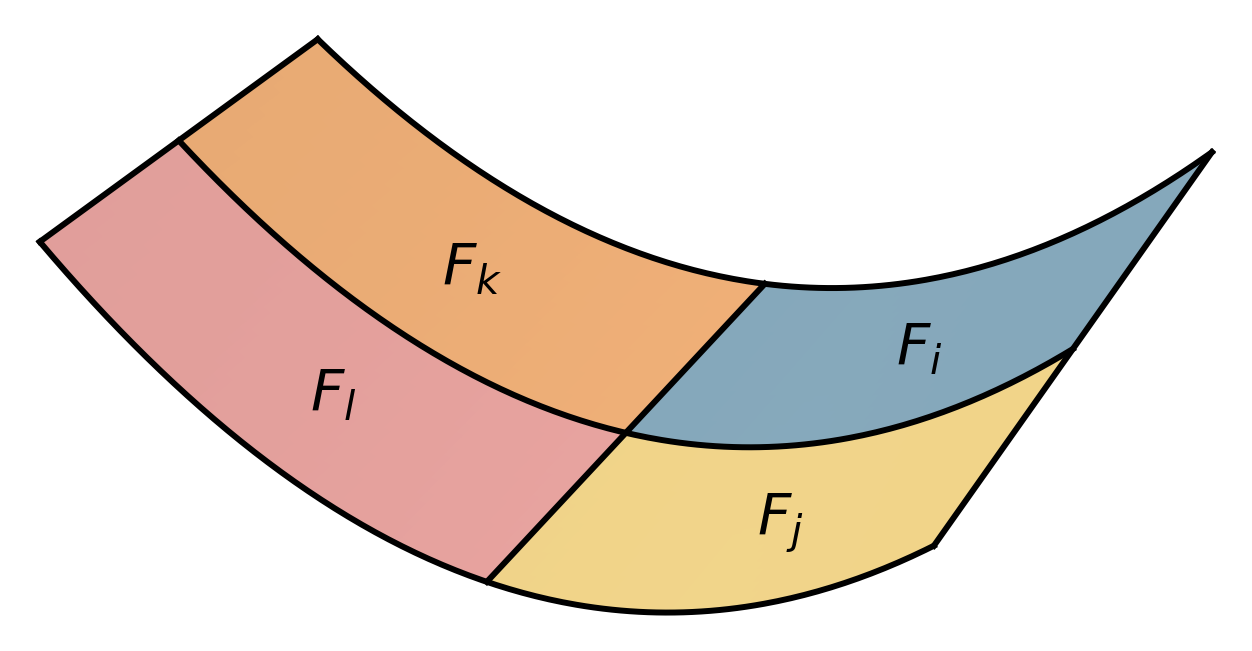
\includegraphics[width=46mm]{figures/fig5_bspline_curved_sheet.png}};
  \node[note] at (29,-37) {Four original B-Rep faces};
  \draw[flow] (54,-20) -- (65,-20);
  \draw[figSixInk!65,line width=.6pt]
    (71,-15) -- (87,-15) -- (87,-27) -- (71,-27) -- cycle;
  \foreach \x/\y/\c/\f in {71/-15/figSixFaceThree/F3,87/-15/figSixFaceOne/F1,71/-27/figSixFaceFour/F4,87/-27/figSixFaceTwo/F2} {
    \node[circle,draw=figSixInk!65,fill=\c,minimum size=6mm,
      line width=.55pt,inner sep=0] at (\x,\y) {\f};
  }
  \node[note] at (79,-37) {Face-adjacency graph};
  \draw[flow] (93,-20) -- (112,-20);
  \node[card,fill=figSixStone!20,minimum width=41mm,minimum height=24mm]
    (input) at (135,-20)
    {Node attributes: $\mathbf{x}_i\in\mathbb{R}^{48}$\\[1.3mm]
     Edge attributes: $\mathbf{e}_{ij}\in\mathbb{R}^{6}$\\[1.3mm]
     Shared graph connectivity};
  \draw[flow] (input.south) -- (135,-44) -- (0,-44) -- (0,-111) -- (7,-111);
  \draw[flow] (0,-73) -- (7,-73);
  \node[note,fill=white,inner sep=.5mm] at (76,-44)
    {Same inputs; independently learned parameters};
  \node[panel] at (2,-48) {(b) Two class-specific branches};

  \foreach \cy/\col/\branch/\k/\score in {-73/figSixRivet/Rivet branch/r/{p_{r,i}},-111/figSixSurface/Surface-feature branch/s/{p_{s,i}}} {
    \draw[groupbox,draw=\col!75!black,fill=\col!5]
      (4,\cy+21) rectangle (154,\cy-15);
    \node[anchor=west,text=\col!65!black,
      font=\sffamily\fontsize{8.2}{9.5}\selectfont] at (7,\cy+17) {\branch};
    \node[card,draw=\col!75,fill=figSixStone!14,
      minimum width=28mm,minimum height=26mm] (enc\k) at (21,\cy) {};
    \node[note] at (21,\cy+9.5) {Node / edge encoders};
    \node[card,fill=figSixPurple!35,draw=figSixInk!30,
      minimum width=22mm,minimum height=5.5mm] at (21,\cy+3) {Node: 48D};
    \node[card,fill=figSixGreen!25,draw=figSixInk!30,
      minimum width=22mm,minimum height=5.5mm] at (21,\cy-3.5) {Edge: 6D};
    \node[note] at (21,\cy-9)
      {Independent weights};

    \node[card,draw=\col!75,fill=\col!9,
      minimum width=29mm,minimum height=26mm] (mp\k) at (57,\cy) {};
    \node[note] at (57,\cy+9.5) {Graph encoding};
    % Reuse the four face identities and adjacency cycle from panel (a).
    \draw[draw=\col!85,line width=.55pt]
      (52,\cy+4.5) -- (62,\cy+4.5) -- (62,\cy-2.5)
      -- (52,\cy-2.5) -- cycle;
    \foreach \dx/\dy/\cc/\f in {-5/4.5/figSixFaceThree/F3,5/4.5/figSixFaceOne/F1,-5/-2.5/figSixFaceFour/F4,5/-2.5/figSixFaceTwo/F2} {
      \node[circle,draw=figSixInk!55,fill=\cc,
        font=\sffamily\fontsize{5.5}{6}\selectfont,
        minimum size=4mm,inner sep=0,line width=.4pt] at (57+\dx,\cy+\dy) {\f};
    }
    \node[note] at (57,\cy-9) {$4\times$ NNConv\\[.6mm]Hidden width: 64};

    \node[card,draw=\col!75,fill=figSixGreen!10,
      minimum width=28mm,minimum height=26mm] (pool\k) at (92,\cy) {};
    \node[note] at (92,\cy+9.5) {Graph pooling};
    \node[card,fill=figSixGreen!25,draw=figSixInk!30,
      minimum width=22mm,minimum height=6mm] at (92,\cy+2) {Mean + Max};
    \node[note] at (92,\cy-7) {Concat local/global\\[.7mm]$64+128\rightarrow192$};

    \node[card,draw=\col!75,fill=figSixYellow!26,
      minimum width=23mm,minimum height=26mm] (head\k) at (122,\cy) {};
    \node[note] at (122,\cy+9.5) {Adapter + head};
    \node at (122,\cy+3) {$192\rightarrow96$};
    \node[note] at (122,\cy-3) {Linear $96\rightarrow1$};
    \node at (122,\cy-9) {Sigmoid $\sigma$};
    \draw[flow] (enc\k.east) -- (mp\k.west);
    \draw[flow] (mp\k.east) -- (pool\k.west);
    \draw[flow] (pool\k.east) -- (head\k.west);
    \node[card,draw=\col!80,fill=\col!22,minimum width=11mm,
      minimum height=12mm] (score\k) at (146,\cy) {$\score$};
    \draw[flow] (head\k.east) -- (score\k.west);
  }

  \node[note] at (77,-129)
    {Graph connectivity is preserved.};
  \node[panel] at (2,-135) {(c) Graph-convolution unit};
  \draw[groupbox,fill=figSixPurple!10] (4,-140) rectangle (102,-176);
  \node[note] at (12,-147) {$\tilde{\mathbf{e}}_{ij,k}$};
  \node[op,fill=figSixYellow!35,minimum width=19mm] (edgeweights) at (29,-147) {Edge MLP};
  \draw[flow] (17,-147) -- (edgeweights.west);
  \node[op,fill=figSixGreen!25,minimum width=29mm] (conditionedweights) at (66,-147)
    {Edge-conditioned weights};
  \draw[flow] (edgeweights.east) -- (conditionedweights.west);
  \node[op,fill=figSixRivet!15,minimum width=18mm] (conv) at (29,-162) {NNConv};
  \draw[flow] (conditionedweights.south) -- (66,-153) -- (29,-153) -- (conv.north);
  \node[op,fill=figSixStone!25,minimum width=9mm] (norm) at (48,-162) {LN};
  \node[op,fill=figSixGreen!25,minimum width=12mm] (relu) at (63,-162) {ReLU};
  \node[op,fill=figSixRose!23,minimum width=16mm] (drop) at (81,-162) {Dropout};
  \node[circle,draw=figSixInk!65,fill=white,minimum size=4mm,inner sep=0] (add) at (96,-162) {$+$};
  \node[note] at (12,-157) {$\mathbf{h}_{i,k}^{(\ell)}$};
  \draw[flow] (7,-162) -- (conv.west);
  \draw[flow] (conv.east) -- (norm.west);
  \draw[flow] (norm.east) -- (relu.west);
  \draw[flow] (relu.east) -- (drop.west);
  \draw[flow] (drop.east) -- (add.west);
  \draw[flow] (add.east) -- (101,-162);
  \draw[flow,draw=figSixRivet] (7,-162) -- (7,-171) -- (96,-171) -- (add.south);
  \node[note,fill=figSixPurple!10,inner sep=.5mm] at (50,-171) {Residual skip: layers 2--4};
  \node[note] at (53,-180)
    {LN: LayerNorm. First layer: $48\rightarrow64$, without a skip.};

  \node[panel] at (109,-135) {(d) Threshold decision};
  \node[card,fill=figSixStone!27,minimum width=47mm,minimum height=14mm]
    (fusion) at (133,-147)
    {Rivet precedence\\$\tau_r=0.9,\quad\tau_s=0.5$};
  \draw[flow,draw=figSixRivet] (scorer.east) -- (158,-73) -- (158,-147) -- (fusion.east);
  \draw[flow,draw=figSixSurface] (scores.south) -- (146,-136) -- (145,-136) -- (145,-140);
  \draw[flow] (fusion.south) -- (133,-157);
  \draw[groupbox,fill=figSixStone!7] (109,-157) rectangle (157,-181);
  \foreach \cy/\col/\label in {-161/figSixStone/Background,-169/figSixRivet/Rivet,-177/figSixSurface/Surface-feature} {
    \node[card,draw=\col!70!black,fill=\col!20,minimum width=41mm,
      minimum height=6mm,inner sep=.5mm] at (133,\cy) {\label};
  }
  \node[note] at (133,-185) {Three-class output};
\end{tikzpicture}
\endgroup
